\section{Faire avancer et reculer le robot}

\index{Paramètre}Nous avons vu au chapitre \ref{ch:proc-pascal} qu'une déclaration de 
procédure permet de donner un nom à une séquence de commandes que le 
\robot\ peut ensuite exécuter une ou plusieurs fois quand on appelle la procédure par son  nom.
Une procédure peut avoir un ou plusieurs {\em paramètres}.  Dans ce cas la procédure
peut réaliser des actions semblables mais différentes quand on l'appelle avec des paramètres
différents.

Par exemple la procédure
 {\idt avf} commande au \robot\ d'\underline{av}ancer tout droit une
ou plusieurs \underline{f}ois de la taille d'un côté d'un carreau du quadrillage.
Elle a un paramètre qui indique le nombre de fois qu'il faut avancer.
En \ocaml, pour appeler une procédure avec un paramètre, on écrit le nom de la procédure suivi
d'un blanc puis de la valeur du paramètre.
`{\idt avf\ 1}' est équivalent à `{\idt av\ ()}' tandis que
`{\idt avf\ 4}' est équivalent à `{\idt av\ ();\ av\ ();\ av\ ();\ av\ ()}'.
Quand le paramètre est nul, la commande `{\idt avf\ 0}' ne fait pas changer le \robot\ de position.
Enfin quand le paramètre est un nombre négatif, c'est-à-dire un nombre précédé du
signe moins $-$, le \robot\ recule du nombre de fois indiqué sans changer d'orientation. Par exemple
`{\idt avf\ ($-$4)}' est équivalent à `{\idt pdt\ ();\ av\ ();\ av\ ();\ av\ ();\ av\ ();\ pdt\ ()}'.

Un nombre négatif doit être placé entre parenthèses. Si l'on écrit `{\idt avf\ $-$4}', le
compilateur comprend que l'on veut soustraire 4 de {\idt avf}, ce qui n'a pas de sens, et 
signale `{\tt The value avf has type int -> unit but an expression was expected of type int}'
(la valeur {\idt avf} est une procédure qui prend un entier alors qu'un entier était attendu).
De même, quand le paramètre est une expression entière, il faut l'écrire entre parenthèses, comme
dans `{\idt avf\ (2\ $\ast$\ j)}'. Sans les parenthèses, `{\idt avf\ 2\ $\ast$\ j}' serait compris comme
`{\idt (avf\ 2)\ $\ast$\ j}', c'est-à-dire la multiplication par {\idt j} du résultat de la 
commande {\idt avf\ 2}, ce qui n'a pas de sens non plus car {\idt (avf\ 2)} n'est pas un nombre entier.

On peut maintenant comprendre les parenthèses vides {\idt ()} qui suivent les commandes
du \robot\ que nous avons utilisées jusqu'ici, comme {\idt av\ ()} ou {\idt pqtd\ ()}~: 
en \ocaml\ une procédure a toujours au moins un paramètre et {\idt ()} est le paramètre
`vide' que l'on donne aux procédures qui n'ont besoin d'aucune information pour s'exécuter.

\begin{exemple}{\rm
 Le programme {\idt StriesOctogonales} ci-dessous dessine les stries triangulaires réparties
 sur les côtés d'un octogone invisible représentées à la figure \ref{fig:stries-oct}
 (page \pageref{fig:stries-oct})~:\hfill
 \pagebreak[3]
 \input ocaml/StriesOctogonales.tex
\noindent $\Box$ }\end{exemple}
\begin{figure}[htbp]
 \includevspacePostScript[6.0cm]{StriesOctogonales}{0.95}{0.95}
 \caption{Stries sur octogone (Échelle $\frac{1}{3}$)}
 \label{fig:stries-oct}
\end{figure}

\section{Épaisseur du crayon}

La commande {\idt ec}  définit l'\underline{é}paisseur du \underline{c}rayon du \robot. 
Son paramètre entier indique l'épaisseur du crayon
qui  est choisie. Jusqu'ici nous avons employé un crayon d'épaisseur 1 qui est celle qu'utilise
le \robot\ par défaut c'est-à-dire quand on ne lui donne pas d'autres précisions. La
commande {\idt ec\ 2} permet de dessiner avec un trait deux fois plus gros. L'unité de
longueur choisie pour mesurer l'épaisseur du crayon est le {\em pixel} c'est-à-dire,
rappelons-le, la
taille du plus petit point qui peut être dessiné sur l'écran de l'ordinateur.

Quand on utilise un très gros crayon, il faut savoir que le crayon du \robot\ 
a une mine carrée et que le \robot\ tient cette mine par son coin supérieur  gauche.
\begin{center}
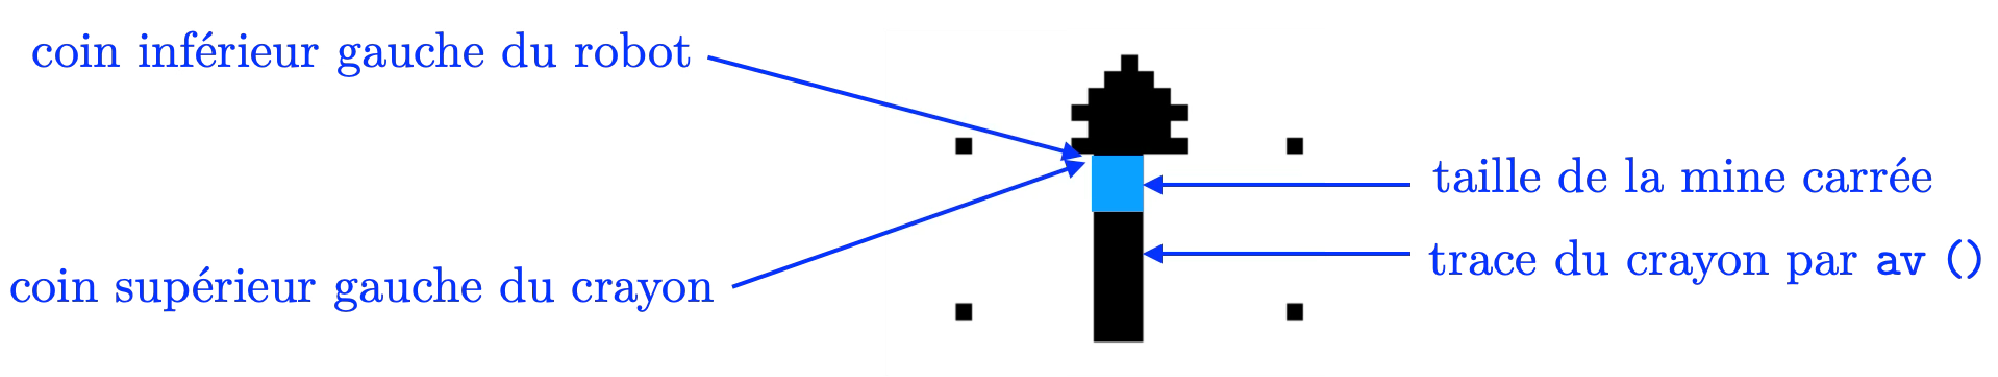
\includegraphics[width=0.9\textwidth]{ps-files/PositionTraceCrayon.pdf}
\end{center}

\begin{exemple}[Crayon à grosse mine]{\rm
Le programme ci-dessous, {\idt EpaisseurCrayon}, permet d'observer
 l'effet de l'exécution d'une commande {\idt av\ ()} avec une grille
 standard de 12 pixels quand le \robot\ utilise des épaisseurs
 successives du crayon de $12$, $24$, $36$ et $48$
 pixels~:\par\nopagebreak
\noindent\begin{minipage}[t][6.4cm][t]{\linewidth}
\vspace*{6cm}%
\includePostScript{EpaisseurCrayon}{0.95}{0.95}%
\vspace*{-6cm}%
\input ocaml/EpaisseurCrayon.tex
\end{minipage}
On observera par exemple que le trait tracé quand le \robot\ exécute
une commande {\idt av\ ()} avec un crayon de 48 pixels a une longueur
apparente de 5 fois la longueur du côté du quadrillage.  Ceci
s'explique par le fait qu'en position finale le crayon laisse une
trace carrée de côté $48$ pixels en bas à droite de son point d'arrêt
soit $4$ fois la longueur du côté du quadrillage de $12$ pixels. 
$\Box$ }%
\end{exemple}

\section{Vitesse du robot}

Un dernier exemple de procédure avec paramètre est la commande {\idt vt} pour choisir
la \underline{v}i\underline{t}esse du \robot. Cette vitesse est un nombre entier compris entre
0 et 10. La vitesse 10 correspond à la vitesse maximale par défaut. Donc la commande {\idt vt\ 10}
est équivalente à la commande {\idt ex\ ()} d'exécution normale. La vitesse
{\idt vt\ 1} correspond à la vitesse minimale. Elle permet d'observer tous les détails des
mouvements du \robot\ qui, à cette vitesse, sont très lents. Enfin la vitesse  0
correspond à l'exécution en mode pas à pas. La commande {\idt vt\ 0} est donc équivalente
à la commande {\idt pp\ ()}. Le mode pas à pas est utilisé pour trouver les erreurs dans les
programmes. Dans ce mode d'exécution, les commandes du \robot\ s'affichent en bas de l'écran
et s'exécutent en tapant sur une touche (ou en cliquant sur le bouton de la souris). Les parcours
du \robot\ avec le crayon levé sont marqués en pointillés ce qui permet de suivre 
parfaitement sa trace.

\noindent \rule{137mm}{0.1mm} %---------------------------------------------
\begin{exercices}{Écrire un programme \ocaml\ pour dessiner~:

\tiret la lettre H majuscule en relief de la figure \ref{fig:h-relief} (page \pageref{fig:h-relief})$\:$;

\tiret le cube en perspective, le cristal à huit branches et la paire de lunettes de la figure \ref{fig:crist+lun} (page \pageref{fig:crist+lun})$\:$;

\tiret l'hélicoptère et le train de voyageurs de la figure \ref{fig:transports} (page \pageref{fig:transports})$\:$;

\tiret les courbes `spirolatérales' de la figure \ref{fig:spiro} (page \pageref{fig:spiro}), obtenues en faisant avancer
le \robot\ une fois puis deux fois puis trois fois, etc., en tournant à chaque fois d'un quart de tour à droite et en répétant
le tout quatre fois de suite (\cite{odds1})$\:$;

\tiret l'arabesque et l'échelle de Jacob de la figure \ref{fig:JacobArab} (page \pageref{fig:JacobArab}), échelle de Jacob que l'on pourra également essayer de
réaliser en entrelaçant une ficelle entre ses doigts.

\noindent $\Box$}\end{exercices}
\begin{figure}[htbp]
 \includevspacePostScript[2.6cm]{Cristal+Lunettes}{0.95}{0.95}
 \caption{Cube en perspective, cristal à huit branches et paire de lunettes}
 \label{fig:crist+lun}
\end{figure}
\begin{figure}[htbp]
 \includevspacePostScript[4.0cm]{Spirolaterales}{0.95}{0.95}
 \caption{Spirolatérales à 90$^{\circ}$ d'ordre 5, 7 et 9}
 \label{fig:spiro}
\end{figure}
\begin{figure}[htbp]
 \includevspacePostScript[4.5cm]{JacobArab}{0.95}{0.95}
 \caption{Arabesque et échelle de Jacob}
 \label{fig:JacobArab}
\end{figure}

\clearpage

\begin{corrige} {\hfill
\input ocaml/Spirolaterale90oDordre9.tex
\noindent $\Box$}\end{corrige}
\nopagebreak
%%%%%%%%%%%%%%%%%%%%%%%%%%%%%%%%%%%%%%%%%%%%%%%%%%%%%%%%%%%%%%%%%%%%%%%%%%%
\noindent \framebox[\textwidth]{
\begin{minipage}{\myparboxwidth}
\setlength{\parindent}{2em}
\small \sf
\vspace{\abovedisplayskip}
\section*{Addenda}
L'usage de paramètres dans les procédures est une des notions de base de la programmation~:
chaque appel de la procédure dépend d'une ou plusieurs valeurs en fonction desquelles on
exprime l'effet de la procédure. Nous ne considérons pour l'instant que le passage de paramètres
{\em par valeur} qui permet de passer une information (un ou plusieurs nombres dans notre cas)
 à une procédure. Ceci rejoint la notion élémentaire de {\em fonction} (ou {\em application}) 
en mathématiques.

L'emploi de sous-programmes avec paramètres en langage machine est généralement attribué à \href{https://en.wikipedia.org/wiki/Alan_Turing}{Alan Turing}. 
Le suisse \href{https://en.wikipedia.org/wiki/Heinz_Rutishauser}{Heinz Rutishauser} \cite{rutishauser} et l'italien
\href{https://en.wikipedia.org/wiki/Corrado_Böhm}{Corrado Böhm} \cite{bohm} introduisirent les notions de langage de programmation évolué et de compilateur
pour traduire les programmes écrits dans ce langage évolué en langage machine (on ne parlait pas à l'époque
de compilateur mais de {\em codification automatique}). Ils incluèrent la notion de sous-programme avec paramètres
dans leurs langages  sans la dégager très explicitement. 

Après ces contributions théoriques liminaires, le premier compilateur qui ait fonctionné sur la machine 
{\sc mark i} à Manchester en Angleterre fût construit par \href{https://en.wikipedia.org/wiki/Alick_Glennie}{Alick Glennie} en 1952. Le language évolué
\href{https://en.wikipedia.org/wiki/Autocode}{{\sc autocode}} utilisait des sous-programmes avec paramètres passés dans les registres de la machine. 

\vspace{\abovedisplayskip}
\end{minipage}
}
%%%%%%%%%%%%%%%%%%%%%%%%%%%%%%%%%%%%%%%%%%%%%%%%%%%%%%%%%%%%%%%%%%%%%%%%%%%%

%%%%%%%%%%%%%%%%%%%%%%%%%%%%%%%%%%%%%%%%%%%%%%%%%%%%%%%%%%%%%%%%%%%%%%%%%%%
\noindent \framebox[\textwidth]{
\begin{minipage}{\myparboxwidth}
\setlength{\parindent}{2em}
\small \sf
\vspace{\abovedisplayskip}
Ce travail
n'eut aucun succès car le travail de programmation était relativement aisé à l'époque comparé aux efforts
nécessaires pour adapter les programmes aux dysfonctionnements de la machine.  
\href{https://en.wikipedia.org/wiki/Maurice_Wilkes}{Maurice Wilkes} \cite{wilkes1} introduisit 
 l'usage de bi\-blio\-thè\-ques de procédures (comme celles que nous utilisons pour les commandes du \robot) en 1951.

 Le premier langage où  ces notions apparurent sous leur forme moderne fut \href{https://en.wikipedia.org/wiki/Fortran}{\sc fortran} ({\sc for}mula
 {\sc tran}slator) conçu en 1954 par une équipe dirigée par \href{https://en.wikipedia.org/wiki/John_Backus}{John Backus} \cite{fortran}. Grâce à de très
 nombreuses modifications qui incorporent les nouveaux concepts de programmation, 
 aux extensions qui prennent en compte
 les architectures  récentes de machines et à la richesse des bibliothèques disponibles,
 ce langage est encore très utilisé pour la programmation scientifique numérique.

\vspace{\abovedisplayskip}
\end{minipage}
}
%%%%%%%%%%%%%%%%%%%%%%%%%%%%%%%%%%%%%%%%%%%%%%%%%%%%%%%%%%%%%%%%%%%%%%%%%%%%
\newpage
\thispagestyle{empty}
